\maketitle

\tableofcontents

\section{Introducing spectral indices for water}
Spectral indices or spectral index (singular) is a term used to define a result of mathematical operation (map algebra, raster algebra, etc.) of two or more band of spectrum from a multispectral imagery \cite{xue2017significant}.

 The most famous one of spectral indices is NDVI (Normalized Difference Vegetation Index). It is the result from the margin of near infrared (NIR) and red band divided by the sum of both, following Equation \ref{eq:ndvi}. This index have many use such as to classify certain land cover: soil, built-up, water, sparse, and dense vegetation. It also can be used to monitor vegetation health and pattern over time. The result of NDVI is an image with a value ranging from -1 to 1 where value below 0 tend to be water, 0 to 0.3 is built-up, soil, and grass while above the 0.4 to be shrub and denser vegetation. Although high value can be used to identify if the vegetation is healthy. Example of the multispectral imagery and NDVI can be seen in Figure \ref{fig:imageNdvi}.

\begin{equation}
	\label{eq:ndvi}
	NDVI = \frac{NIR - RED}{NIR + RED}
\end{equation}

\begin{figure}[htbp]
	\label{fig:imageNdvi}
	\centering
	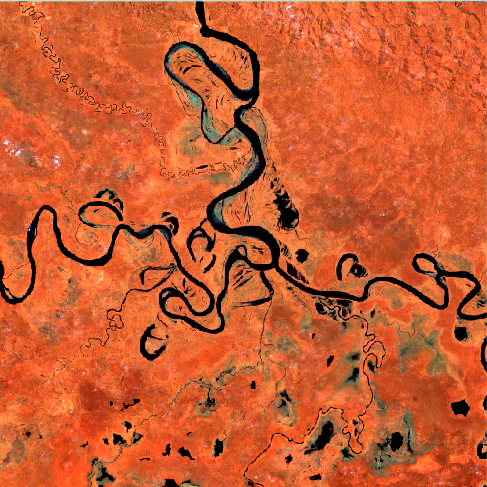
\includegraphics[height=40ex]{komposit.png}
	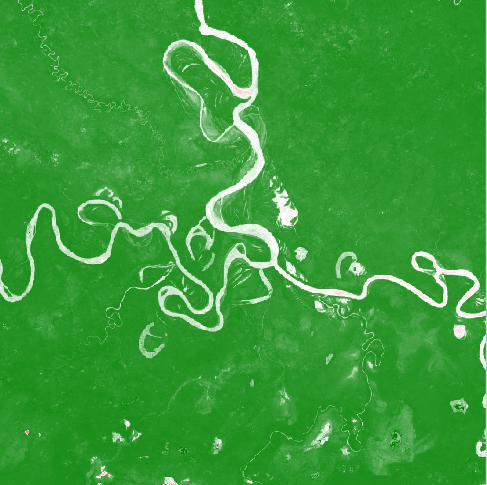
\includegraphics[height=40ex]{ndvi.png}
	\caption{NIR-SWIR1-SWIR2 composite (left) and NDVI (right) image}
\end{figure}

NIR band is used in the formula is following the spectral reflectance curve on how the interaction between multiple electomagnetic wavelength to certain object. This relation could be understand from Figure \ref{fig:spectralCurve}. Based on the curve, it can be understood that the reflectance of vegetation at its peak in NIR band wavelength interval while it have a smaller reflectance in the red spectrum while red band also have a high reflectance in soil object.

\begin{figure}[htbp]
	\label{fig:spectralCurve}
	\centering
	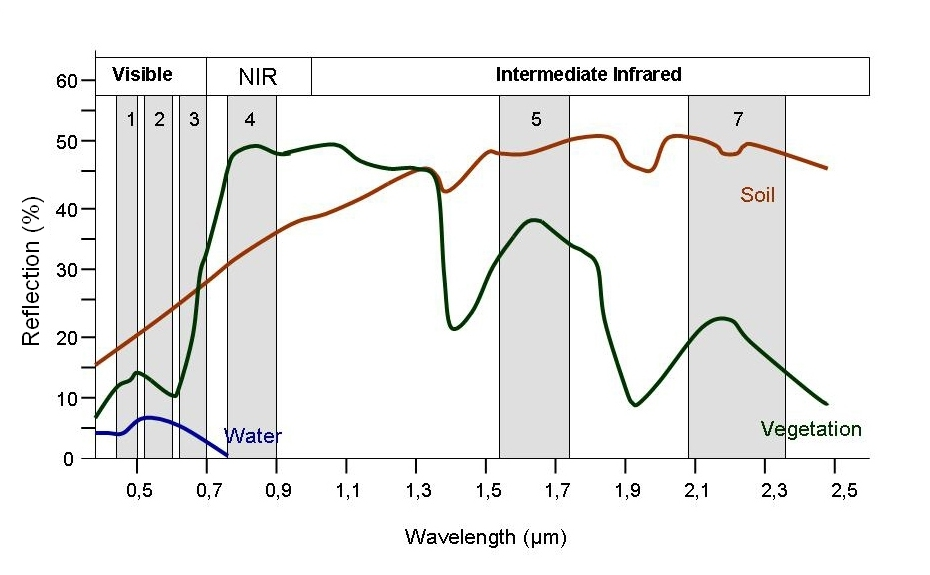
\includegraphics[width=80ex]{Reflexionskurven.jpg}
	\caption{Spectral reflectance curve of soil, vegetation, and water on multiple electromagnetic spectrum \cite{siegmund2005fernes}}
\end{figure}

While NDVI is quite famous and used for vegetation, spectral indices can also be used for many type of objects. NDWI (Normalized Difference Water Index) is one of the indices used to help identify water object \cite{gao1996ndwi}. It used near-infrared (NIR) and green wavelengths. NIR infrared is known to have reflectance on multiple objects (soil and vegetation) and low on water. While, green wavelength is known to reflect highly of water object, even more than blue wavelength. Using the normalized difference between the band follow Equation \ref{eq:ndwi}, it allow us to calculate how wet or closesly resemblance to water the area is.

\begin{equation}
	\label{eq:ndwi}
	NDWI = \frac{GREEN - NIR}{GREEN + NIR}
\end{equation}

Figure \ref{fig:ndwi} show the comporison of Landsat NIR-SWIR1-SWIR2 composite and NDWI. It can be seen that water area in Landsat composite, represented in black color is colored white to blue to in NDWI, which it mean it can differenciate between water and other object.

\begin{figure}[htbp]
	\label{fig:ndwi}
	\centering
	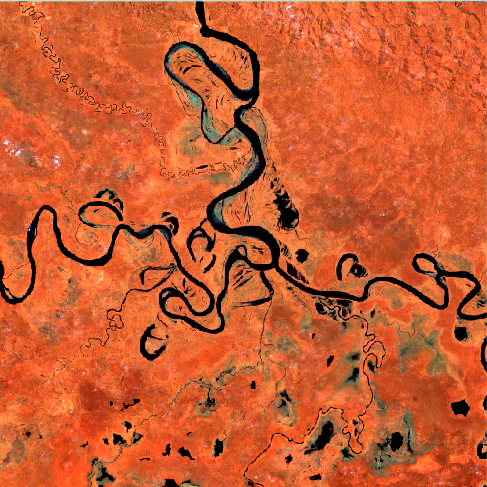
\includegraphics[height=40ex]{komposit.png}
	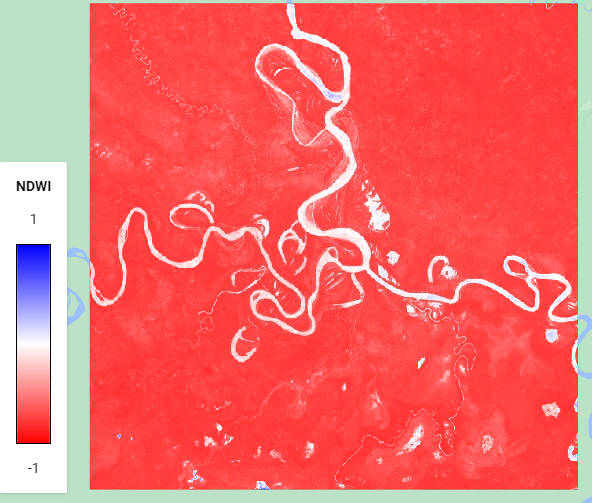
\includegraphics[height=40ex]{ndwi.png}
	\caption{Comparison of Landsat NIR-SWIR1-BLUE composite (left) and NDWI (right)}
\end{figure}

NDWI is not the only water indices, there are many more such as MNDWI (Modified Normalized Difference Water Index) and NDMI (Normalized Difference Mositure Index). MNDWI is using short wavelength infrared band with following Equation \ref{eq:mndwi}.

\begin{equation}
	\label{eq:mndwi}
	MNDWI = \frac{GREEN - SWIR1}{GREEN + SWIR1}
\end{equation}

\section{Calculating water spectral indices in Google Earth Engine}
Google Earth Engine (GEE) is cloud-based geospatial analysis software for global scale and multitemporal data \cite{gorelick2017google}. It is allow user to do analysis online without the need for high computation resources. It is also store many remote sensing data that can be use directly. This allow professionals and academics to utilize for many project and research.

Calculating spectral indices is one method to analyze the landscape using multispectral satellite imagery. This imagery are available in the GEE, so instead of downloading the image then calculate the indices in a GIS software, is it now posibble to do it directly in the cloud. 

In GEE, an imagery or stack of multispectral imagery is represented by \verb|ee.Image| object/class. This object will have several properties such as all the bands of stacked image inside, geometry boundary, date, source, and any other properties. Using the bands available in the \verb|ee.Image|, it is possible to calculate built-up indices. It could be done using mathematical operation such as \verb|add, subtract, multiply, & divide| or using \verb|ee.Image.expression| method where it receive two arguments: the formula in quoted text/string and band map or the definition of the formula's variables. Script \ref{code:expression} show the example to calculate MNDWI using Landsat composite imagery.

\begin{lstlisting}[language=JavaScript, label={code:expression}, caption={GEE script to calculate NDWI from Landsat 8 and 9 composite}]
// Landsat 8 and 9 collection
var landsat8 = ee.ImageCollection("LANDSAT/LC08/C02/T1_L2");
var landsat9 = ee.ImageCollection("LANDSAT/LC09/C02/T1_L2");

// ROI
var geometry = ee.Geometry({
	"geodesic": false,
	"type": "Polygon",
	"coordinates": [
		[
			[
				138.25184277142827,
				-3.0784162244028095
			],
			[
				138.58692577924077,
				-3.0784162244028095
			],
			[
				138.58692577924077,
				-2.7451378202231855
			],
			[
				138.25184277142827,
				-2.7451378202231855
			],
			[
				138.25184277142827,
				-3.0784162244028095
			]
		]
	]
});

// Parameter
var roi = geometry;
var start = '2022-01-31';
var end = '2022-12-31';

// Function for cloud masking
function cloudMasking(image){
	var qa = image.select('QA_PIXEL');
	var dilated = 1 << 1;
	var cirrus = 1 << 2;
	var cloud = 1 << 3;
	var shadow = 1 << 4;
	var mask = qa.bitwiseAnd(dilated).eq(0)
		.and(qa.bitwiseAnd(cirrus).eq(0))
		.and(qa.bitwiseAnd(cloud).eq(0))
		.and(qa.bitwiseAnd(shadow).eq(0));
	return image.updateMask(mask).select(['SR_B.*'], ['B1', 'B2', 'B3', 'B4', 'B5', 'B6', 'B7']) // Select only important band
		.multiply(0.0000275).add(-0.2); // Scale the value to 0 - 1
}

// Get image from collection
var image = landsat8.filterBounds(roi) // Filter by geometry
	.filterDate(start, end) // Filter by date
	.merge(landsat9.filterBounds(roi).filterDate(start, end)) // Merge with landsat 9 collection
	.map(cloudMasking) // Apply cloud mask
	.median() // Median composite
	.clip(roi); // Clip the image

// Show image
Map.addLayer(image, { min: [0.1, 0.05, 0.025], max: [0.4, 0.3, 0.2], bands: ['B5', 'B6', 'B7'] }, 'Image');

// Band map
var bandMap = {
	SWIR1: image.select('B6'),
	GREEN: image.select('B3'),
};

// MNDWI
var mndwi = image.expression('MNDWI = (GREEN - SWIR1) / (GREEN + SWIR1)', bandMap);
Map.addLayer(mndwi, { min: -1, max: 1, palette: ['red', 'white', 'blue'] }, 'MNDWI');
\end{lstlisting}

\section{Modelling water body using relational operation}
NDWI is an index that show a value from -1 to 1 where value closer to 1 have high probability to be a water and it is fewer when approaching -1. Therefore it is possible to get water body or classify water body using certain threshold of NDWI. The threshold can be changed based on the temporal, region, and type of satellite used. 

In the region of interest, a small section in Papua Island, the value is above 0, it is due to high concentration of sediment in the water. If it in other region that is not considered sediment, the value can be set higher, to not make less watery object to be considered water.

Threshold determination can be done using relational operation in GEE, we could determine the condition to decice built-up area. In GEE, relational operation can be done using \verb|lt, lte, gt, gte, eq, neq, and, or|, where each will state if our threshold is lower than (\verb|lt|) or greater than (\verb|gte|) of certain value. Script \ref{code:relational} show how to classify built-up area using relational operation which utilize some indices. It also using Landsat NIR band to mask cloud. The result can be seen in Figure \ref{fig:water}.

\begin{lstlisting}[language=JavaScript, label={code:relational}, caption={GEE Script to Classify Water using Relational Operation}]
// Water object
var water = mndwi.gte(0);
Map.addLayer(water.selfMask(), { palette: 'blue' }, 'Water');
\end{lstlisting}

\begin{figure}[htbp]
	\label{fig:water}
	\centering
	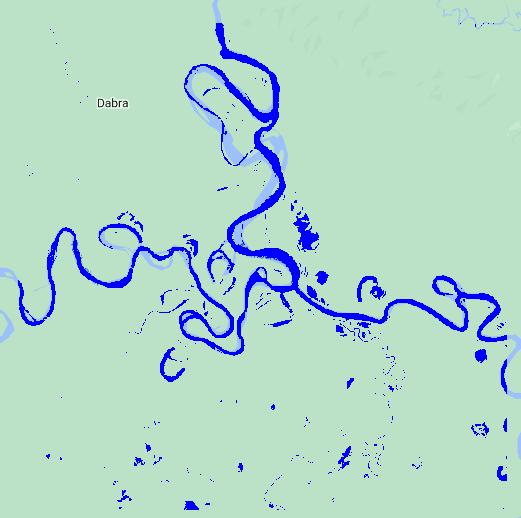
\includegraphics[width=50ex]{water.png}
	\caption{Water object clasified using relational operation of MNDWI}
\end{figure}

\section{Modelling river change using multitemporal data}
It is possible to apply the relational operation in multi years to see the river flow change over year. It can done using image collection \verb|ee.ImageCollection| and loop operation using \verb|map|. Each water object in each year can a value using it year where reducer operation \verb|reducer| can do \verb|ee.Reducer.min| method to the collection to put earlier value on top of other data to see the change. Script \ref{code:riverChange} is an example how to do that from year 1990 to 2020. The result will be like Figure \ref{fig:riverChange}.

\begin{lstlisting}[language=JavaScript, label={code:riverChange}, caption={GEE script to model river change}]
// Landsat 8 and 9 collection
var landsat4 = ee.ImageCollection("LANDSAT/LT04/C02/T1_L2");
var landsat5 = ee.ImageCollection("LANDSAT/LT05/C02/T1_L2");
var landsat7 = ee.ImageCollection("LANDSAT/LE07/C02/T1_L2");
var landsat8 = ee.ImageCollection("LANDSAT/LC08/C02/T1_L2");
var landsat9 = ee.ImageCollection("LANDSAT/LC09/C02/T1_L2");

// ROI
var geometry = ee.Geometry({
	"geodesic": false,
	"type": "Polygon",
	"coordinates": [
		[
			[
				138.25184277142827,
				-3.0784162244028095
			],
			[
				138.58692577924077,
				-3.0784162244028095
			],
			[
				138.58692577924077,
				-2.7451378202231855
			],
			[
				138.25184277142827,
				-2.7451378202231855
			],
			[
				138.25184277142827,
				-3.0784162244028095
			]
		]
	]
});

// Parameter
var roi = geometry;
var start = '2022-01-31';
var end = '2022-12-31';

// Function to filter
function filterCol(col, roi, date){
  return col.filterDate(date[0], date[1]).filterBounds(roi);
}

// Composite function
function landsat457(roi, date){
  var col = filterCol(landsat4, roi, date).merge(filterCol(landsat5, roi, date)).merge(filterCol(landsat7, roi, date));
  var image = col.map(cloudMaskTm).median().clip(roi);
  return image;
}

function landsat89(roi, date){
  var col = filterCol(landsat8, roi, date).merge(filterCol(landsat9, roi, date));
  var image = col.map(cloudMaskOli).median().clip(roi);
  return image;
}

// Cloud mask
function cloudMaskTm(image){
  var qa = image.select('QA_PIXEL');
  var dilated = 1 << 1;
  var cloud = 1 << 3;
  var shadow = 1 << 4;
  var mask = qa.bitwiseAnd(dilated).eq(0)
    .and(qa.bitwiseAnd(cloud).eq(0))
    .and(qa.bitwiseAnd(shadow).eq(0));
  
  return image.select(['SR_B1', 'SR_B2', 'SR_B3', 'SR_B4', 'SR_B5', 'SR_B7'], ['B2', 'B3', 'B4', 'B5', 'B6', 'B7']).updateMask(mask);
}

function cloudMaskOli(image){
  var qa = image.select('QA_PIXEL');
  var dilated = 1 << 1;
  var cirrus = 1 << 2;
  var cloud = 1 << 3;
  var shadow = 1 << 4;
  var mask = qa.bitwiseAnd(dilated).eq(0)
    .and(qa.bitwiseAnd(cirrus).eq(0))
    .and(qa.bitwiseAnd(cloud).eq(0))
    .and(qa.bitwiseAnd(shadow).eq(0));
  
  return image.select(['SR_B2', 'SR_B3', 'SR_B4', 'SR_B5', 'SR_B6', 'SR_B7'], ['B2', 'B3', 'B4', 'B5', 'B6', 'B7']).updateMask(mask);
}

var yearList = [1990, 1995, 2000, 2005, 2010, 2015, 2020];

// Generate image per year
var waterCol = ee.ImageCollection(yearList.map(function(year){
  var start = ee.Date.fromYMD(year - 1 , 1, 1);
  var end = ee.Date.fromYMD(year + 1, 12, 31);
  var date = [start, end];
  
  // Conditional on landsat collection to use
  var landsat;
  if (year < 2014) {
    landsat = landsat457;
  } else {
    landsat = landsat89;
  }
  
  // Create an image composite
  var image = landsat(roi, date).multiply(0.0000275).add(-0.2);
  
  // Show the image
  Map.addLayer(image, { min: [0.1, 0.05, 0.025], max: [0.4, 0.3, 0.2], bands: ['B5', 'B6', 'B7'] }, 'Landsat_' + year, false);
  
  // Band map
  var bandMap = { 
    NIR: image.select('B5'), 
    SWIR: image.select('B6'), 
    RED: image.select('B4'), 
    GREEN: image.select('B3'), 
    BLUE: image.select('B2') 
  };
  
  // Modified Normalized Difference Water Index
  var mndwi = image.expression('(GREEN - SWIR) / (GREEN + SWIR)', bandMap).rename('MNDWI');
  
  // Show the MNDWI
  Map.addLayer(mndwi, { min: -1, max: 1, palette: ['red', 'white', 'blue'] }, 'MNDWI_' + year, false);
  
  // Built up
  var water = mndwi.gt(0.1).selfMask().multiply(year).toInt();
  Map.addLayer(water, { palette: 'blue' }, 'Water_' + year, false);
  
  return water.rename('water').set('year', year, 'system:time_start', start);
}));

// Create dictionary for each year expansion for visualization
var dict = {
  'water_class_values': yearList,
  'water_class_palette': ['800080', '0000FF', '00FFFF', '008000', 'FFFF00', 'FFA500', 'FF0000']
};

// Create river change iamge
var riverChange = waterCol.min().set(dict);
Map.addLayer(riverChange, {}, 'River change');
\end{lstlisting}

\begin{figure}[htbp]
	\label{fig:riverChange}
	\centering
	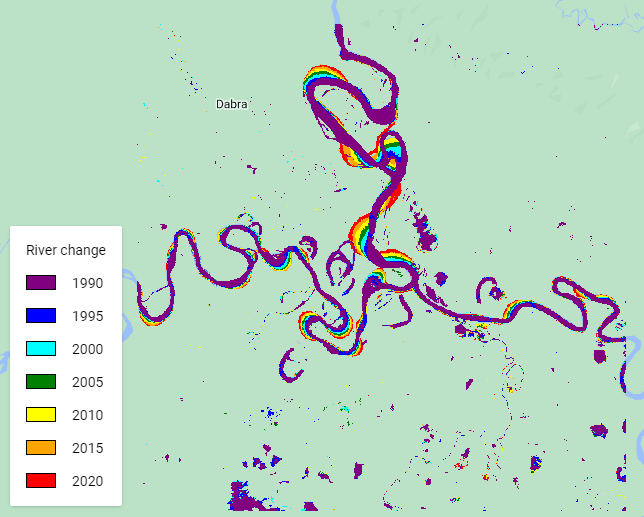
\includegraphics[width=50ex]{riverChange.png}
	\caption{River change modelling using multitemporal data}
\end{figure}

\section{Modelling coastline change change using multemporal data}
Modelling water over time is not only can be used to see the change in the river but any body of water. Using the same principle, this method allow us to model coastline change over the years. Intead of masking the water object, it is the other way around, where we could classify land area, assuming this area is the coast. Script \ref{code:coastlineChange} show you how to model coastline change using Google Earth Engine. The result will look like Figure \ref{fig:coastlineChange}.

\begin{lstlisting}[language=JavaScript, label={code:coastlineChange}, caption={GEE script to model coastline change}]
// Geometry 2
var geometry2 = ee.Geometry({
  "geodesic": false,
  "type": "Polygon",
  "coordinates": [
    [
      [
        107.93123947814016,
        -6.347125408772628
      ],
      [
        108.09191452696828,
        -6.347125408772628
      ],
      [
        108.09191452696828,
        -6.228367833844507
      ],
      [
        107.93123947814016,
        -6.228367833844507
      ],
      [
        107.93123947814016,
        -6.347125408772628
      ]
    ]
  ]
});

// Geometry
var roi = geometry2;

// Year list
var yearList = [1990, 1995, 2000, 2005, 2010, 2015, 2020];

// Generate image per year
var landCol = ee.ImageCollection(yearList.map(function(year){
  var start = ee.Date.fromYMD(year - 1 , 1, 1);
  var end = ee.Date.fromYMD(year + 1, 12, 31);
  var date = [start, end];
  
  // Conditional on landsat collection to use
  var landsat;
  if (year < 2014) {
    landsat = landsat457;
  } else {
    landsat = landsat89;
  }
  
  // Create an image composite
  var image = landsat(roi, date).multiply(0.0000275).add(-0.2);
  
  // Show the image
  Map.addLayer(image, { min: [0.1, 0.05, 0.025], max: [0.4, 0.3, 0.2], bands: ['B5', 'B6', 'B7'] }, 'Landsat_' + year, false);
  
  // Band map
  var bandMap = { 
    NIR: image.select('B5'), 
    SWIR: image.select('B6'), 
    RED: image.select('B4'), 
    GREEN: image.select('B3'), 
    BLUE: image.select('B2') 
  };
  
  // Modified Normalized Difference Water Index
  var mndwi = image.expression('MNDWI = (GREEN - SWIR) / (GREEN + SWIR)', bandMap);
  
  // Show the MNDWI
  //Map.addLayer(mndwi, { min: -1, max: 1, palette: ['red', 'white', 'blue'] }, 'MNDWI_' + year, false);
  
  // Built up
  var land = mndwi.lte(0.1).selfMask().multiply(year).toInt();
  Map.addLayer(land, { palette: 'burlywood' }, 'Land_' + year, false);
  
  return land.rename('land').set('year', year, 'system:time_start', start);
}));

// Create dictionary for each year expansion for visualization
var dict = {
  'land_class_values': yearList,
  'land_class_palette': ['800080', '0000FF', '00FFFF', '008000', 'FFFF00', 'FFA500', 'FF0000']
};

// Costaline change
var coastlineChange = landCol.max().set(dict);
Map.addLayer(coastlineChange, {}, 'Coastline change change');
\end{lstlisting}

\begin{figure}[htbp]
	\label{fig:coastlineChange}
	\centering
	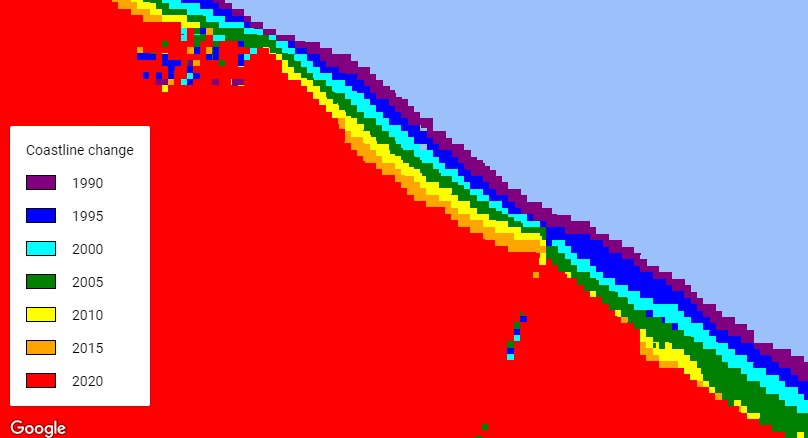
\includegraphics[height=40ex]{coastlineChange.png}
	\caption{Coastline change from multiple years}
\end{figure}

\section{Introducing remote sensing for coastal and benthic habitat}
Remote sensing is a tool to observe many phenomenon in the Earth without directly in contact with said phenomenon. Most of remote sensing activity is about natural resources in the land area such as agriculture and forestry. Most famous and publicly used remote sensing satellite is used to said research. However it is also used to observe underwater object, although not the so deep one.

Benthic habitat mapping is one of the type of remote sensing usage to map object underwater. Benthic is a term to describe a region in intertidal zone (zone of tidal between land and sea) (Figure \ref{fig:benthic}). It is the shallow part of the sea where some optical electromagnetic wavelength can still penetrate such as coastal, blue, green, and red band, where it stil can reflect some object as seen in Figure \ref{fig:spectralCurve}.

\begin{figure}[htbp]
	\label{fig:benthic}
	\centering
	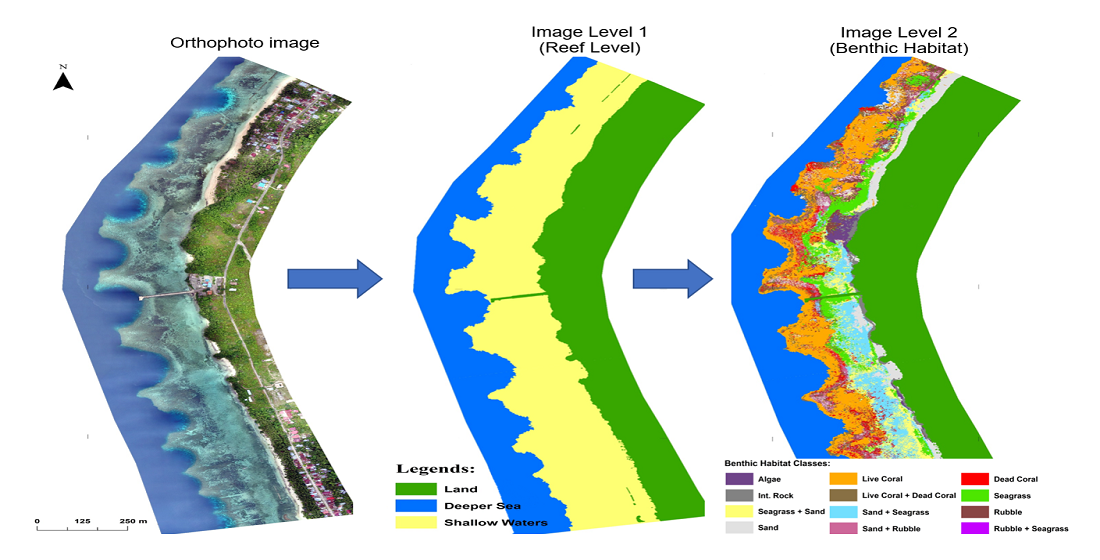
\includegraphics[height=40ex]{benthic.png}
	\caption{Benthic zone \cite{nababan2021shallow}}	
\end{figure}

Object that can be mapped in benthic zone usually are coral reef, seagrass, sand, rubble, and algae. You can visit \url{https://allencoralatlas.org/atlas/#13.12/-8.2993/116.7022} to view Allen Coral Atlas, a global map of coral reef and which also include other benthic habitat.

\section{Sunglint and below surface correction for Sentinel-2 image}
It is uncommon to map benthic habitat directly, to enchance and expose the benthic habitat more, it usually need certain correction. There are many correction to use like sunglint and below surface correction.

Before correction, it is important to mask the important area, which is the benthic habitat zone. This can be done using water indices like NDWI and MNDWI \cite{gao1995normalized}. Using certain threshold, it can mask the area for further analysis.

Sunglint correction is method to correct the actual reflectance of underwater object that usually covered by high sun beam like in Figure \ref{fig:sunglint}. There are many method to eliminate sunglint but the easiest one is using the subtraction of all visual band with NIR band following Equation \ref{eq:sunglint}.

\begin{equation}
	\label{eq:sunglint}
	SR' = SR_v - SR_{NIR}
\end{equation}

\begin{tabular}{l l l}
	$SR'$ & $=$ & Corrected sunglint reflectance \\
	$SR_v$ & $=$ & Visual band reflectance \\
	$SR_NIR$ & $=$ & NIR band reflectance \\
\end{tabular}

\begin{figure}[htbp]
	\label{fig:sunglint}
	\centering
	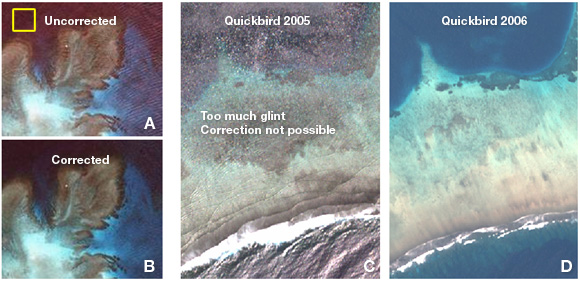
\includegraphics[height=40ex]{sunglint.jpg}
	\caption{Sunglint and Sunglint Correction Result \cite{hedley2005simple}}
\end{figure}

After sunglint correction, it also possible to get the below surface (underwater) reflectance using Coral Atlas method \cite{li2019adaptive}. This method allow us to increase the reflectance of underwater object and certainly help in mapping shallow bathymetry and benthic habitat. Equation \ref{eq:belowSurface} show you how to accomplish that.

\begin{equation}
	\label{eq:belowSurface}
	BSR = \frac{SR}{0.52 + 1.7 * SR}
\end{equation}

\begin{tabular}{l l l}
	$BSR$ & $=$ & Below surface reflectance \\
	$SR$ & $=$ & Visual band reflectance \\
\end{tabular}

The whole step from selecting image, benthic masking, sunglint correction, and below surface reflectance can be followed in Script \ref{code:preprocessing}. We are using Sentinel-2 image, the highest resolution multispetral imagery publicly available where we are only using the 10 meter bands: RGB and NIR. The visualization of each step can be seen in Figure \ref{fig:correction}.

\begin{lstlisting}[language=JavaScript, label={code:preprocessing}, caption={GEE script for multiple benthic correction}]
// Sentine-2 collection
var s2 = ee.ImageCollection("COPERNICUS/S2_SR_HARMONIZED");

// Geometry data
var geometry = ee.Geometry({
	"geodesic": false,
	"type": "Polygon",
	"coordinates": [
		[
			[
				116.67848403575506,
				-8.314655032688776
			],
			[
				116.71968276622381,
				-8.314655032688776
			],
			[
				116.71968276622381,
				-8.27303785876449
			],
			[
				116.67848403575506,
				-8.27303785876449
			],
			[
				116.67848403575506,
				-8.314655032688776
			]
		]
	]
});

// Parameter
var roi = geometry;
var start = '2022-01-01';
var end = '2022-12-31';

// Image
var image = s2.filterBounds(roi) //Filter by area
	.filterDate(start, end) // Filter by date
	.sort('CLOUDY_PIXEL_PERCENTAGE') // Sort by cloud cover percentage
	.first() // Get the first image
	.select(['B2', 'B3', 'B4', 'B8']) // Select needed band
	.clip(roi) // Clip to roi
	.divide(10000); // Scale 0 - 1
	
// Show image
Map.addLayer(image, { min: 0, max: 0.15, bands: ['B4', 'B3', 'B2'] }, 'Image');

// NDWI
var ndwi = image.expression('NDWI = (GREEN - NIR) / (GREEN + NIR)', {
	NIR: image.select('B8'),
	GREEN: image.select('B3')
});
Map.addLayer(ndwi, { min: -1, max: 1, palette: ['red', 'white', 'blue'] }, 'NDWI');

// Benthic mage
var benthicImage = image.updateMask(ndwi.gt(0));
Map.addLayer(benthicImage, { min: 0, max: 0.15, bands: ['B4', 'B3', 'B2'] }, 'Benthic Image');

// Corrected sunglint
var sunglintCorrection = benthicImage.select(['B2', 'B3', 'B4'])
	.subtract(benthicImage.select(['B8']));
Map.addLayer(sunglintCorrection, { min: 0, max: 0.15, bands: ['B4', 'B3', 'B2'] }, 'Corrected Sunglint Image');

// Below surface reflectance
var belowSurface = sunglintCorrection.divide(sunglintCorrection.multiply(1.7).add(0.52));
Map.addLayer(belowSurface, { min: 0, max: 0.15, bands: ['B4', 'B3', 'B2'] }, 'Below surface reflectance');
\end{lstlisting}

\begin{figure}[htbp]
	\label{fig:correction}
	\centering
	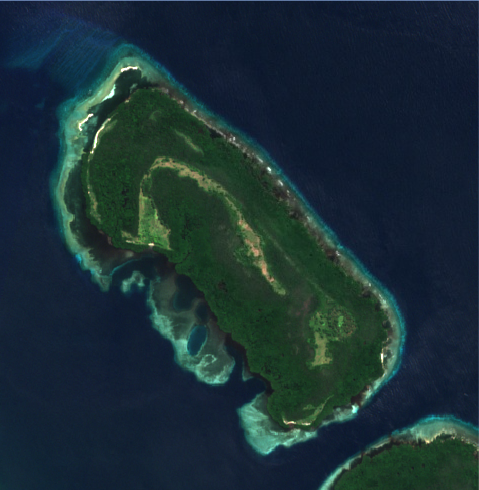
\includegraphics[height=40ex]{benthicImage.png}
	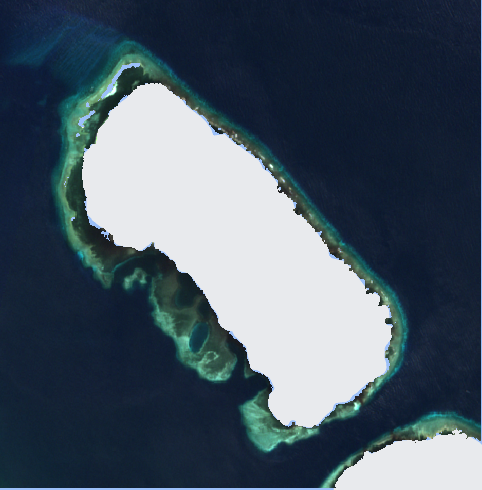
\includegraphics[height=40ex]{benthicMasked.png}
	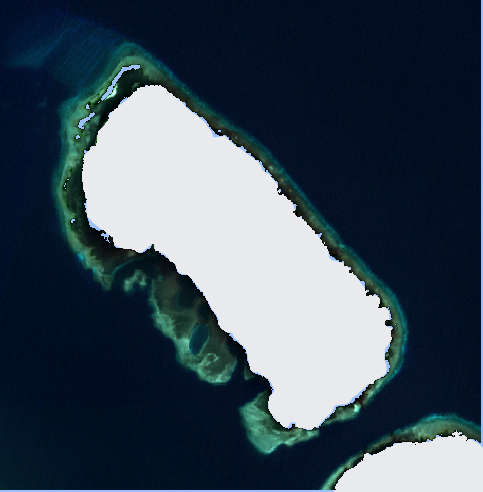
\includegraphics[height=40ex]{sunglintImage.png}
	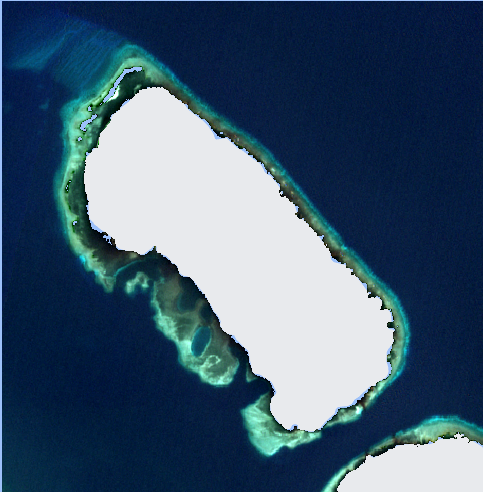
\includegraphics[height=40ex]{belowSurface.png}
	\caption{Surface reflectance image (top-left); Masked using NDWI (top-right); Sunglint corrected (bottom-left); Below surface reflectance (bottom-right)}
\end{figure}

\section{Bathmetry mapping}
Using below surface image, it is possible to map bathymetry with some limitation (not so deep ocean). Following paper \cite{li2021automated}, we can calculate the depth of underwater region using Equation \ref{eq:bathymetry}. Follow Script \ref{code:bathymetry} to accomplish that in GEE. The result will be like Figure \ref{fig:bathymetry}.

\begin{equation}
	\label{eq:bathymetry}
	Depth = m_0 * \frac{\ln(1000 * BLUE)}{\ln(1000 * GREEN)} - m_1
\end{equation}

\begin{tabular}{l l l}
	$Depth$ & $=$ & Sea depth \\
	$m_0$ & $=$ & $52.073 * e^{0.957 * Chl_a} $ \\
	$m_1$ & $=$ & $50.156 * e^{0.957 * Chl_a} $ \\
	$BLUE$ & $=$ & Blue band reflectance \\
	$GREEN$ & $=$ & Green band reflectance \\
\end{tabular}

\begin{lstlisting}[language=JavaScript, label={code:bathymetry}, caption={GEE script to map bathymetry}]
// Calculate depth
var depth = ee.Image().expression('(m0 * (log(1000 * blue) / log(1000 * green))) - m1', {
	m0: ee.Number(52.073).multiply(ee.Number(2.71).pow(0.957 * 0.5)),
	m1: ee.Number(50.156).multiply(ee.Number(2.71).pow(0.957 * 0.5)),
	blue: belowSurface.select('B2'),
	green: belowSurface.select('B3')
}).multiply(-1);
Map.addLayer(depth, { min: 10, max: -40, palette: ['white', 'lightskyblue', 'blue', 'navy'] }, 'Depth');
\end{lstlisting}

\begin{figure}[htbp]
	\label{fig:bathymetry}
	\centering
	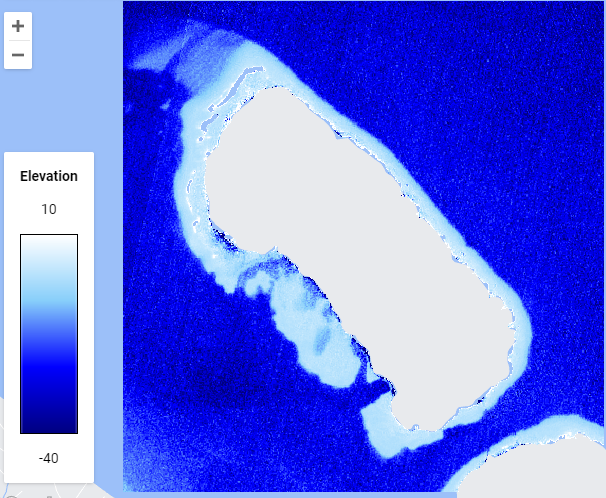
\includegraphics[height=40ex]{bathymetry.png}
	\caption{Elevation in meter above sea level}
\end{figure}

\section{Benthic habitat classification}
The application of using below surface reflectance imagery, other than bathymetry, can also to map benthic habitat such as coral reef, seagrass, sand, rubble, etc. To do that is almost the same when mapping land cover where you have to take sample, create a machine learning model, do accuracy assessment, and apply the model to the image. 

The huge obstacle usually the ability of interpretator to knwo which habitat is which. This need experience and understading the morphology of benthic zone. Using previous below surface image, we can follow Script \ref{code:classify} to map benthic habitat. The result will look like Figure \ref{fig:classify}.

\begin{lstlisting}[language=JavaScript, label={code:classify}, caption={GEE script to map benthic habitat}]
// Sample
var sample = ee.FeatureCollection([
  deep_sea, coral, sand, rubble, seagrass, 
]).flatten();

// Extract sample
var extract = belowSurface.sampleRegions({
  collection: sample,
  scale: 10,
  properties: ['classvalue']
}).randomColumn();

// Split train and test
var train = extract.filter(ee.Filter.lte('random', 0.8));
var test = extract.filter(ee.Filter.gt('random', 0.8));

// Model
var model = ee.Classifier.smileRandomForest(50).train(train, 'classvalue', ['B4', 'B3', 'B2']);

// Assss model
var cm = test.classify(model, 'prediction').errorMatrix('classvalue', 'prediction');
print('Confusion matrix', cm, 'Accuracy', cm.accuracy(), 'Kappa', cm.kappa());

// Legend
var palette = ['FFC0CB', '7FFFD4', 'FFA500', '006400', '000080'];
var names = ['Coral', 'Sand', 'Rubble', 'Seagrass', 'Deep sea'];
var values = [1, 2, 3, 4, 5];

// Benthic
var benthic = belowSurface.classify(model, 'benthic').set({
  'benthic_class_values': values,
  'benthic_class_palette': palette
});
Map.addLayer(benthic, {}, 'Benthic');
\end{lstlisting}

\begin{figure}[htbp]
	\label{fig:classify}
	\centering
	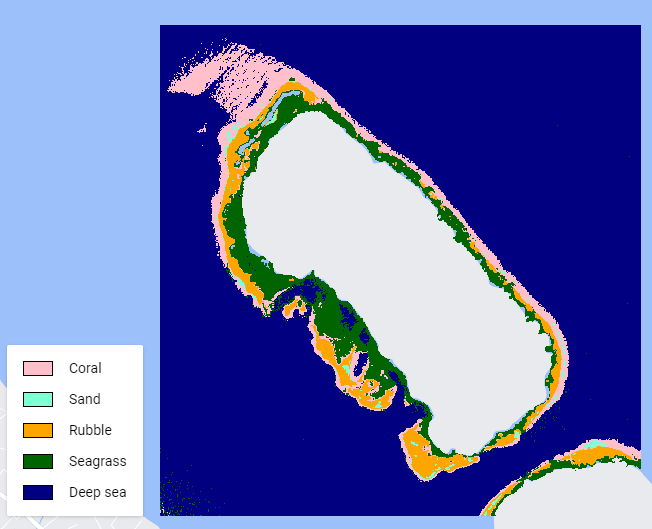
\includegraphics[height=40ex]{benthicHabitat.png}
	\caption{Classifierd benthic habitat}
\end{figure}

\printbibliography